\documentclass[10pt,a4paper]{article}
\usepackage[margin=20mm]{geometry}
\usepackage[T1]{fontenc}
\usepackage{lmodern}
\usepackage{microtype}
\usepackage{tikz}
\usetikzlibrary{positioning,calc,arrows.meta}
\usepackage[hidelinks]{hyperref}
\usepackage{caption}
\usepackage{booktabs}
\usepackage{tabularx}
\usepackage{array}
\captionsetup{font=small,labelfont=bf}
\setlength{\parindent}{1em}
\setlength{\parskip}{3pt}

\begin{document}

\section{Related Work}
\subsection{Classification of Facility Layout Problems and Solution Approaches}

Facility layout research can be organised by problem characteristics,
objective criteria, layout representations, formulation and solution approaches,
spatial configurations, constraints, and data and assessment requirements.
Figure~\ref{fig:flp-framework} summarises these dimensions through a
literature-based classification. The taxonomy synthesises the perspectives of
Drira et al.\ \cite{drira2007}, P\'{e}rez-Gosende et al.\ \cite{perez2021},
Anjos and Vieira\ \cite{anjos2017}, Ahmadi et al.\ \cite{ahmadi2017},
and Liu\ \cite{liu2004}. The dimensions are complementary: an individual
study may combine several characteristics and methods. This selective synthesis
organises the reviewed contributions; it is not an exhaustive taxonomy of all
FLP variants or a systematic review of recent algorithmic developments.

\begin{figure}[htbp]
\centering
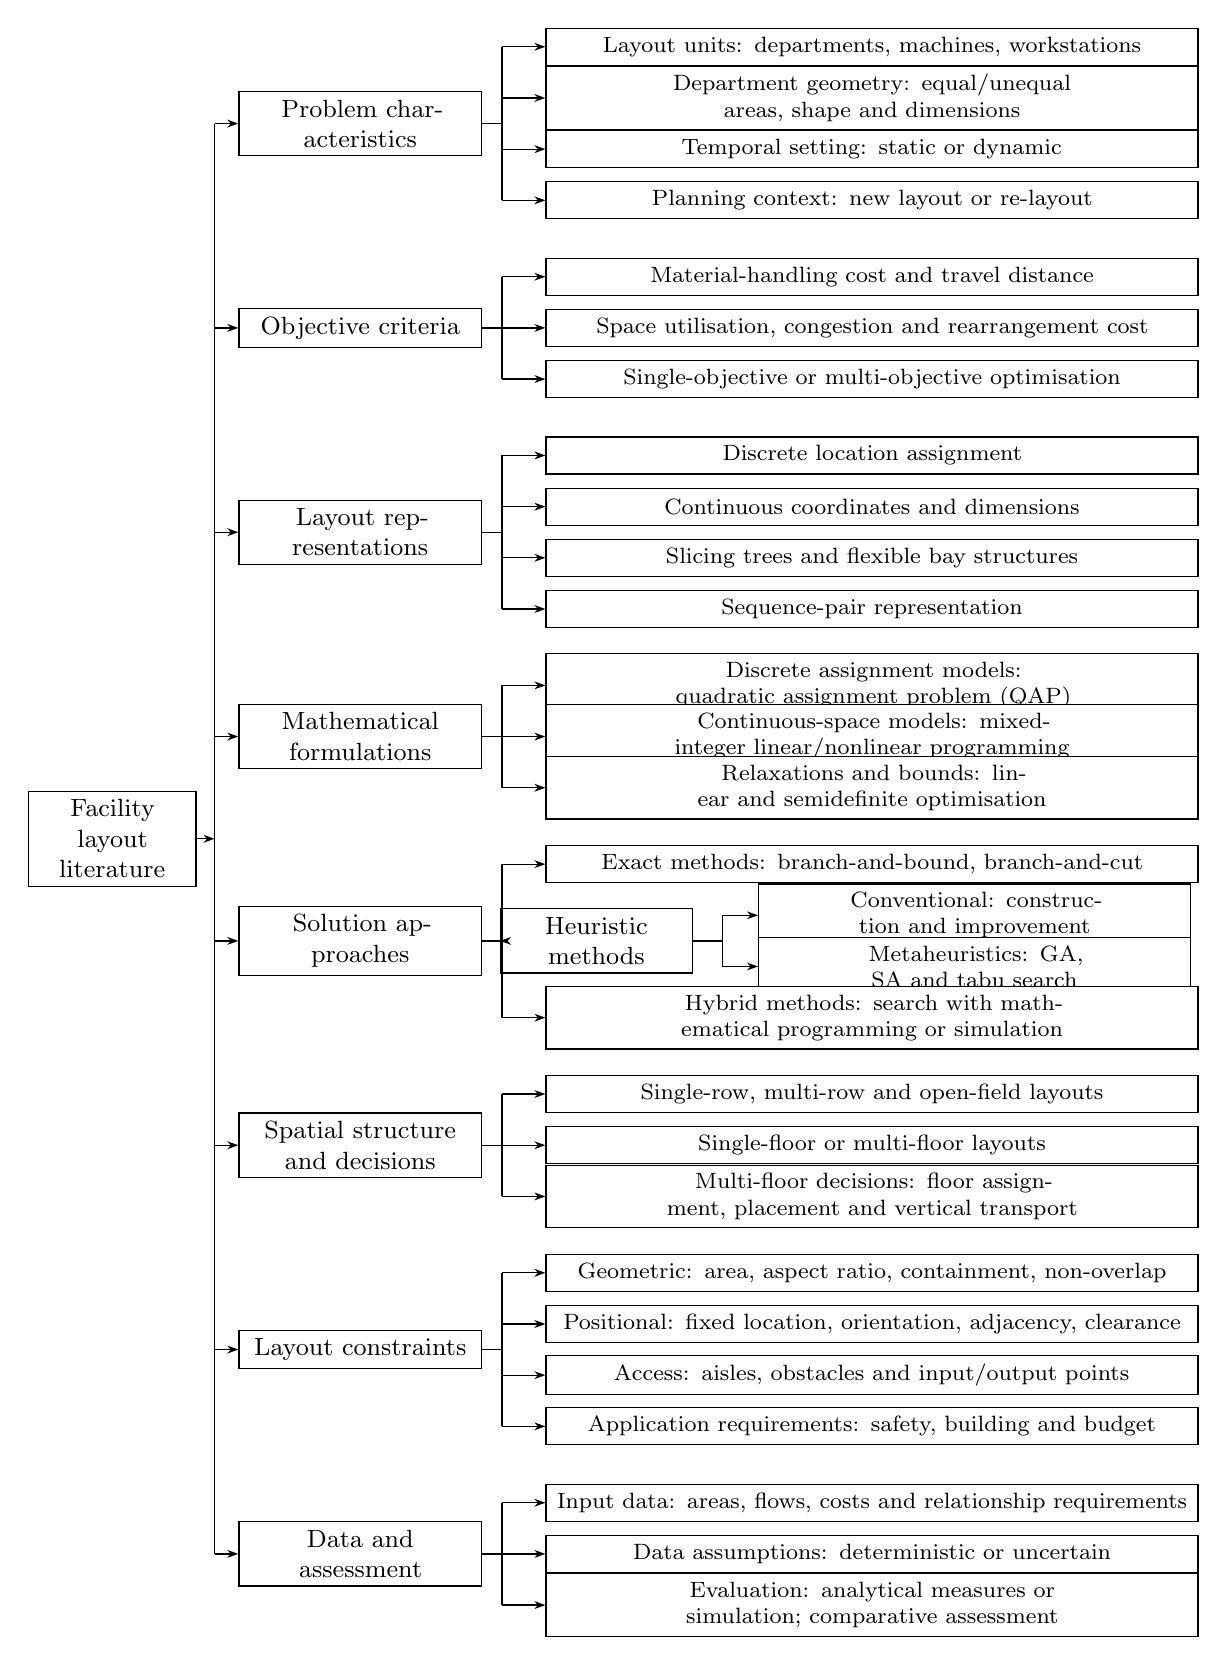
\begin{tikzpicture}[
  box/.style={draw=black,fill=white,line width=.45pt,rectangle,
    align=center,inner xsep=4pt,inner ysep=3pt,font=\small},
  root/.style={box,text width=1.85cm},
  category/.style={box,text width=2.8cm},
  leaf/.style={box,text width=8.0cm,minimum height=.47cm,font=\footnotesize},
  link/.style={draw=black,line width=.45pt,-{Stealth[length=1.4mm,width=1.0mm]}}
]
\node[leaf] (l11) at (9.65,0.000) {Layout units: departments, machines, workstations};
\node[leaf] (l12) at (9.65,-0.650) {Department geometry: equal/unequal areas, shape and dimensions};
\node[leaf] (l13) at (9.65,-1.300) {Temporal setting: static or dynamic};
\node[leaf] (l14) at (9.65,-1.950) {Planning context: new layout or re-layout};
\node[category] (c1) at (3.15,-0.975) {Problem characteristics};
\node[leaf] (l21) at (9.65,-2.920) {Material-handling cost and travel distance};
\node[leaf] (l22) at (9.65,-3.570) {Space utilisation, congestion and rearrangement cost};
\node[leaf] (l23) at (9.65,-4.220) {Single-objective or multi-objective optimisation};
\node[category] (c2) at (3.15,-3.570) {Objective criteria};
\node[leaf] (l31) at (9.65,-5.190) {Discrete location assignment};
\node[leaf] (l32) at (9.65,-5.840) {Continuous coordinates and dimensions};
\node[leaf] (l33) at (9.65,-6.490) {Slicing trees and flexible bay structures};
\node[leaf] (l34) at (9.65,-7.140) {Sequence-pair representation};
\node[category] (c3) at (3.15,-6.165) {Layout representations};
\node[leaf] (l41) at (9.65,-8.110) {Discrete assignment models: quadratic assignment problem (QAP)};
\node[leaf] (l42) at (9.65,-8.760) {Continuous-space models: mixed-integer linear/nonlinear programming};
\node[leaf] (l43) at (9.65,-9.410) {Relaxations and bounds: linear and semidefinite optimisation};
\node[category] (c4) at (3.15,-8.760) {Mathematical formulations};
\node[leaf] (l51) at (9.65,-10.380) {Exact methods: branch-and-bound, branch-and-cut};
\node[box,text width=2.15cm] (l52) at (6.15,-11.355) {Heuristic methods};
\node[leaf,text width=5.2cm] (l52a) at (10.95,-11.030) {Conventional: construction and improvement};
\node[leaf,text width=5.2cm] (l53) at (10.95,-11.680) {Metaheuristics: GA, SA and tabu search};
\node[leaf] (l54) at (9.65,-12.330) {Hybrid methods: search with mathematical programming or simulation};
\node[category] (c5) at (3.15,-11.355) {Solution approaches};
\node[leaf] (l61) at (9.65,-13.300) {Single-row, multi-row and open-field layouts};
\node[leaf] (l62) at (9.65,-13.950) {Single-floor or multi-floor layouts};
\node[leaf] (l63) at (9.65,-14.600) {Multi-floor decisions: floor assignment, placement and vertical transport};
\node[category] (c6) at (3.15,-13.950) {Spatial structure and decisions};
\node[leaf] (l71) at (9.65,-15.570) {Geometric: area, aspect ratio, containment, non-overlap};
\node[leaf] (l72) at (9.65,-16.220) {Positional: fixed location, orientation, adjacency, clearance};
\node[leaf] (l73) at (9.65,-16.870) {Access: aisles, obstacles and input/output points};
\node[leaf] (l74) at (9.65,-17.520) {Application requirements: safety, building and budget};
\node[category] (c7) at (3.15,-16.545) {Layout constraints};
\node[leaf] (l81) at (9.65,-18.490) {Input data: areas, flows, costs and relationship requirements};
\node[leaf] (l82) at (9.65,-19.140) {Data assumptions: deterministic or uncertain};
\node[leaf] (l83) at (9.65,-19.790) {Evaluation: analytical measures or simulation; comparative assessment};
\node[category] (c8) at (3.15,-19.140) {Data and assessment};
\node[root] (root) at (0,-10.058) {Facility layout\\literature};
\draw[link] (root.east) -- (1.3,0 |- root.east);
\draw[black,line width=.45pt] (1.3,-0.975) -- (1.3,-19.140);
\draw[link] (1.3,0 |- c1.west) -- (c1.west);
\draw[black,line width=.45pt] (c1.east) -- (4.95,-0.975);
\draw[black,line width=.45pt] (4.95,0 |- l11.west) -- (4.95,0 |- l14.west);
\draw[link] (4.95,0 |- l11.west) -- (l11.west);
\draw[link] (4.95,0 |- l12.west) -- (l12.west);
\draw[link] (4.95,0 |- l13.west) -- (l13.west);
\draw[link] (4.95,0 |- l14.west) -- (l14.west);
\draw[link] (1.3,0 |- c2.west) -- (c2.west);
\draw[black,line width=.45pt] (c2.east) -- (4.95,-3.570);
\draw[black,line width=.45pt] (4.95,0 |- l21.west) -- (4.95,0 |- l23.west);
\draw[link] (4.95,0 |- l21.west) -- (l21.west);
\draw[link] (4.95,0 |- l22.west) -- (l22.west);
\draw[link] (4.95,0 |- l23.west) -- (l23.west);
\draw[link] (1.3,0 |- c3.west) -- (c3.west);
\draw[black,line width=.45pt] (c3.east) -- (4.95,-6.165);
\draw[black,line width=.45pt] (4.95,0 |- l31.west) -- (4.95,0 |- l34.west);
\draw[link] (4.95,0 |- l31.west) -- (l31.west);
\draw[link] (4.95,0 |- l32.west) -- (l32.west);
\draw[link] (4.95,0 |- l33.west) -- (l33.west);
\draw[link] (4.95,0 |- l34.west) -- (l34.west);
\draw[link] (1.3,0 |- c4.west) -- (c4.west);
\draw[black,line width=.45pt] (c4.east) -- (4.95,-8.760);
\draw[black,line width=.45pt] (4.95,0 |- l41.west) -- (4.95,0 |- l43.west);
\draw[link] (4.95,0 |- l41.west) -- (l41.west);
\draw[link] (4.95,0 |- l42.west) -- (l42.west);
\draw[link] (4.95,0 |- l43.west) -- (l43.west);
\draw[link] (1.3,0 |- c5.west) -- (c5.west);
\draw[black,line width=.45pt] (c5.east) -- (4.95,-11.355);
\draw[black,line width=.45pt] (4.95,0 |- l51.west) -- (4.95,0 |- l54.west);
\draw[link] (4.95,0 |- l51.west) -- (l51.west);
\draw[link] (4.95,0 |- l52.west) -- (l52.west);
\draw[black,line width=.45pt] (l52.east) -- (7.75,0 |- l52.east);
\draw[black,line width=.45pt] (7.75,0 |- l52a.west) -- (7.75,0 |- l53.west);
\draw[link] (7.75,0 |- l52a.west) -- (l52a.west);
\draw[link] (7.75,0 |- l53.west) -- (l53.west);
\draw[link] (4.95,0 |- l54.west) -- (l54.west);
\draw[link] (1.3,0 |- c6.west) -- (c6.west);
\draw[black,line width=.45pt] (c6.east) -- (4.95,-13.950);
\draw[black,line width=.45pt] (4.95,0 |- l61.west) -- (4.95,0 |- l63.west);
\draw[link] (4.95,0 |- l61.west) -- (l61.west);
\draw[link] (4.95,0 |- l62.west) -- (l62.west);
\draw[link] (4.95,0 |- l63.west) -- (l63.west);
\draw[link] (1.3,0 |- c7.west) -- (c7.west);
\draw[black,line width=.45pt] (c7.east) -- (4.95,-16.545);
\draw[black,line width=.45pt] (4.95,0 |- l71.west) -- (4.95,0 |- l74.west);
\draw[link] (4.95,0 |- l71.west) -- (l71.west);
\draw[link] (4.95,0 |- l72.west) -- (l72.west);
\draw[link] (4.95,0 |- l73.west) -- (l73.west);
\draw[link] (4.95,0 |- l74.west) -- (l74.west);
\draw[link] (1.3,0 |- c8.west) -- (c8.west);
\draw[black,line width=.45pt] (c8.east) -- (4.95,-19.140);
\draw[black,line width=.45pt] (4.95,0 |- l81.west) -- (4.95,0 |- l83.west);
\draw[link] (4.95,0 |- l81.west) -- (l81.west);
\draw[link] (4.95,0 |- l82.west) -- (l82.west);
\draw[link] (4.95,0 |- l83.west) -- (l83.west);
\end{tikzpicture}
\caption{A synthesis of facility layout classifications and methodological
choices in the reviewed literature \cite{drira2007,perez2021,anjos2017,ahmadi2017,liu2004}.
Branches indicate analytical dimensions; method families may overlap.
GA: genetic algorithm; SA: simulated annealing.}
\label{fig:flp-framework}
\end{figure}
\clearpage
\subsection{Problem Characteristics, Objectives and Constraints}

The first dimension identifies what is being arranged and under which planning
conditions. Functional units, such as machining, assembly and storage areas,
must be distinguished from their geometric properties. A storage department
may be rectangular, fixed in position, or distributed over several floors;
these properties introduce different modelling requirements. General FLP
classifications also distinguish static and dynamic planning and the design of
new facilities from the rearrangement of existing ones\ \cite{drira2007,perez2021}.
Consequently, an algorithm should be selected against an explicitly defined
problem, rather than against a department's functional label alone.

The second dimension defines how layout quality is measured. Material-handling
cost and travel distance are common criteria, but a project's objectives may
also include space use, operational performance and the cost of future
rearrangement\ \cite{drira2007,perez2021}. Multiple criteria require an explicit
decision rule, such as a justified weighted objective or the comparison of
non-dominated alternatives. A shorter geometric distance should not automatically
be interpreted as improved operational performance when transport capacity,
queues or route restrictions are omitted from the evaluation.

Constraints define the admissible layouts. Area requirements, shape limits,
containment and non-overlap determine geometric feasibility, while fixed
locations, access requirements and aisle structures impose additional practical
conditions\ \cite{anjos2017,liu2004}. Adjacency and separation should be specified
explicitly where needed: positive material flow alone does not require two
departments to share a boundary. Building and safety requirements are application-dependent and must be
translated into explicit restrictions when relevant to the case under study.

\subsection{Representation, Formulation and Solution Methods}

Layout representation describes how a candidate arrangement is encoded.
Coordinates and dimensions describe geometry directly, whereas slicing trees,
flexible bay structures and sequence-pairs encode spatial structure or relative
order\ \cite{anjos2017,liu2004}. The representation affects which arrangements
can be explored and how they are decoded. In particular, a structural encoding
must not be assumed to cover every feasible geometric layout without examining
its restrictions.

Mathematical formulation specifies decision variables, objective functions and
constraints. Discrete location assignment is commonly expressed through the
quadratic assignment problem (QAP). Continuous-space layouts instead determine
coordinates and dimensions, often using mixed-integer linear or nonlinear
programming formulations. Relaxations, including linear and semidefinite
optimisation models, provide bounds that support mathematical optimisation
and solution assessment\ \cite{anjos2017}. A relaxation does not generally
produce a feasible layout for the original problem, and its bound must be
distinguished from the cost of a feasible candidate.

Performance evaluation is a separate concern. Analytical distance and cost
functions may be sufficient for a simplified model, while simulation can assess
transport, queues and congestion\ \cite{perez2021,ahmadi2017}. Simulation by
itself evaluates a candidate rather than specifying how new layouts are
searched; it can therefore be coupled with an optimisation procedure.

Solution methods determine how the encoded or formulated problem is explored.
Exact algorithms can establish optimality when their search and bounds are
sufficient, whereas construction, improvement and metaheuristic methods seek
useful solutions without a general guarantee of global optimality\ \cite{drira2007}.
Construction and improvement procedures can be distinguished from general
metaheuristic search strategies, although both belong to the broader family
of heuristic methods.
Hybrid methods combine complementary components. For example, Liu searches
sequence-pairs using a genetic algorithm and combines this search with
mathematical programming to determine department geometry\ \cite{liu2004}.
Representation, formulation and solution are therefore connected choices,
not three competing alternatives.

\subsection{Spatial Structure, Multi-Floor Effects and Assessment}

Multiple floors couple department-to-floor assignment with the arrangement
within each floor. Vertical transport introduces additional decisions and costs,
including the placement and use of lifts\ \cite{ahmadi2017}. A favourable
within-floor arrangement may consequently be unattractive when its inter-floor
flows are considered. Clear height, structural loading and usable area are
application-dependent engineering requirements. Their inclusion varies with
the building and the scope of the layout model.

The reviewed classifications also distinguish the data assumptions under which
layouts are generated and assessed\ \cite{drira2007,perez2021}. In addition to
area and material-flow data, formulations may use cost parameters, qualitative
relationship requirements, and deterministic or uncertain demand assumptions.
This distinction matters when comparing reported results: methods evaluated
under different objectives, distance definitions or geometric restrictions
are not directly comparable. A consistent comparison should therefore state
the instance data and feasibility conditions, and report solution quality and
computational effort. Repeated runs are also relevant when stochastic search
methods are assessed.

\subsection{Comparison of the Reviewed Contributions}

The cited works contribute at different levels (Table~\ref{tab:review-comparison}).
Drira et al.\ \cite{drira2007} provide a broad classification of problem
conditions and approaches. P\'{e}rez-Gosende et al.\ \cite{perez2021}
extend the planning perspective to the generation and assessment of layout
alternatives. Anjos and Vieira\ \cite{anjos2017} examine mathematical
formulations and optimisation techniques, while Ahmadi et al.\ \cite{ahmadi2017}
focus specifically on multi-floor problems. Liu\ \cite{liu2004} contributes a
concrete methodology that combines representation, search and mathematical
programming. These contributions should therefore be compared by their scope
and decision coverage, rather than treated as interchangeable algorithm studies.

\begin{table}[htbp]
\centering
\caption{Scope and relevance of the selected literature.}
\label{tab:review-comparison}
\small
\renewcommand{\arraystretch}{1.16}
\begin{tabularx}{\textwidth}{@{}p{.17\textwidth} >{\raggedright\arraybackslash}X >{\raggedright\arraybackslash}X@{}}
\toprule
\textbf{Source} & \textbf{Principal contribution} & \textbf{Use and interpretation boundary} \\
\midrule
Drira et al.\ \cite{drira2007}
& General classification of FLP characteristics, formulations and solution approaches.
& Establishes terminology and problem dimensions; does not provide a common ranking of algorithms for the present project. \\
\addlinespace
P\'{e}rez-Gosende et al.\ \cite{perez2021}
& Extended review of planning conditions and the generation and assessment of alternatives.
& Connects optimisation to planning and evaluation; the review's coverage is not a matched computational experiment across all methods. \\
\addlinespace
Anjos and Vieira\ \cite{anjos2017}
& Mathematical optimisation formulations, relaxations and solution techniques.
& Supports model selection and bounds; applicability depends on the geometry and assumptions of each formulation. \\
\addlinespace
Ahmadi et al.\ \cite{ahmadi2017}
& Multi-floor problem characteristics, modelling and solution approaches.
& Identifies floor assignment and vertical-transport considerations; results for single-floor layouts cannot be assumed to transfer unchanged. \\
\addlinespace
Liu\ \cite{liu2004}
& Sequence-pair search combined with mathematical programming, with extensions for fixed departments, aisles and non-rectangular departments.
& Demonstrates a concrete hybrid methodology; extensions require their corresponding geometric restrictions and repair procedures. \\
\bottomrule
\end{tabularx}
\end{table}

This comparison motivates a requirement-driven selection of methods: the
representation must accommodate the target layouts, the formulation must
capture their geometric and operational restrictions, and the search method
must be evaluated under comparable computational conditions. The present
synthesis supports this selection but does not establish a universally superior
algorithm. In particular, any extension to multiple floors requires an explicit
account of floor assignment and inter-floor transport rather than relying solely
on the quality of a two-dimensional layout.

\begin{thebibliography}{9}
\bibitem{drira2007}
A. Drira, H. Pierreval, and S. Hajri-Gabouj,
``Facility layout problems: A survey,''
\textit{Annual Reviews in Control}, vol. 31, no. 2, pp. 255--267, 2007,
doi: \href{https://doi.org/10.1016/j.arcontrol.2007.04.001}{10.1016/j.arcontrol.2007.04.001}.

\bibitem{perez2021}
P. P\'{e}rez-Gosende, J. Mula, and M. D\'{i}az-Madro\~nero,
``Facility layout planning. An extended literature review,''
\textit{International Journal of Production Research}, vol. 59, no. 12,
pp. 3777--3816, 2021,
doi: \href{https://doi.org/10.1080/00207543.2021.1897176}{10.1080/00207543.2021.1897176}.

\bibitem{anjos2017}
M. F. Anjos and M. V. C. Vieira,
``Mathematical optimization approaches for facility layout problems:
The state-of-the-art and future research directions,''
\textit{European Journal of Operational Research}, vol. 261, no. 1,
pp. 1--16, 2017,
doi: \href{https://doi.org/10.1016/j.ejor.2017.01.049}{10.1016/j.ejor.2017.01.049}.

\bibitem{ahmadi2017}
A. Ahmadi, M. S. Pishvaee, and M. R. Akbari Jokar,
``A survey on multi-floor facility layout problems,''
\textit{Computers \& Industrial Engineering}, vol. 107, pp. 158--170, 2017,
doi: \href{https://doi.org/10.1016/j.cie.2017.03.015}{10.1016/j.cie.2017.03.015}.

\bibitem{liu2004}
Q. Liu, ``A sequence-pair and mixed integer programming based methodology
for the facility layout problem,'' Ph.D. dissertation, Dept. Ind. Syst. Eng.,
Virginia Polytechnic Institute and State University, Blacksburg, VA, USA, 2004.
[Online]. Available:
\url{https://vtechworks.lib.vt.edu/server/api/core/bitstreams/34c76035-26bc-4ee1-a580-86711cd7b4c9/content}
\end{thebibliography}

\end{document}
